


%----------------------------------
\chapter{Introduction}\label{ch:SolarBetaintro}
%----------------------------------

\section{Purpose and Objectives of the \SolarBetaDescT}
%%%%%%%%%%%%%%%%%%%%%%%%%%%%%%%%%%%%%%%%%%%%%%%%%%%%%%%%%%%%%%%%%%%%%%%%%%%%%%%%%
%
% Purpose:  Introduction for the SolarBeta model.
%
% 
%
%%%%%%%%%%%%%%%%%%%%%%%%%%%%%%%%%%%%%%%%%%%%%%%%%%%%%%%%%%%%%%%%%%%%%%%%%%%%%%%%


%\section{Purpose and Objectives of \SolarBetaDesc}
% Incorporate the intro paragraph that used to begin this Chapter here. 
% This is location of the true introduction where you explain what this model 
% does.

Spacecraft with movable solar panels and thermal radiators
continuously rotate the solar panels to catch as much sunlight as possible
and rotate the thermal radiators to catch as little sunlight as possible.
The varying orientations of these devices present ever changing cross sections
to atmospheric drag. Properly modeling the orientation of these devices
improves the fidelity of simulation of such spacecraft.

One of the principal drivers of these panel orientations is the angle between
the vector toward the sun and the spacecraft's orbital plane, which is called
the {\em solar beta angle}. The \SolarBetaDesc\ represents this angle.

This part of the document describes the \SolarBetaDesc\ developed for use with \JEODid.

















%----------------------------------
\chapter{Product Requirements}\label{ch:SolarBetareqt}
%----------------------------------


%%%%%%%%%%%%%%%%%%%%%%%%%%%%%%%%%%%%%%%%%%%%%%%%%%%%%%%%%%%%%%%%%%%%%%%%%%%%%%%%%
%
% Purpose:  requirements for the SolarBeta model
%
% 
%
%%%%%%%%%%%%%%%%%%%%%%%%%%%%%%%%%%%%%%%%%%%%%%%%%%%%%%%%%%%%%%%%%%%%%%%%%%%%%%%%

% add text here to describe general model requirements
% text is of the form:
\requirement{Solar Beta representation}
\label{reqt:SolarBeta}
\begin{description}
  \item[Requirement:]\ \newline
     The Solar Beta Derived State will provide the capability for calculating the Solar Beta angle associated with the vehicle's current state.
  \item[Rationale:]\ \newline
     Capability from JEOD 1.5.
  \item[Verification:]\ \newline
     Test
\end{description}

\section{Requirements Traceability}

\begin{longtable}[c]{||p{3.5in}|p{3.5in}|}
\caption{Requirements Traceability} \\[6pt]
\hline
{\bf Requirement} & {\bf Inspection and Testing} \\ 
\hline \hline
\endhead
\ref{reqt:SolarBeta} - Solar Beta representation &
  Test~\ref{test:solarbetalongterm} \\ 
  & Test~\ref{test:solarbetacompare} \\ \hline

\end{longtable}




%----------------------------------
\chapter{Product Specification}\label{ch:SolarBetaspec}
%----------------------------------

\section{Conceptual Design}
%%%%%%%%%%%%%%%%%%%%%%%%%%%%%%%%%%%%%%%%%%%%%%%%%%%%%%%%%%%%%%%%%%%%%%%%%%%%%%%%%
%
% Purpose:  Conceptual part of Product Spec for the SolarBeta model
%
% 
%
%%%%%%%%%%%%%%%%%%%%%%%%%%%%%%%%%%%%%%%%%%%%%%%%%%%%%%%%%%%%%%%%%%%%%%%%%%%%%%%%


%\section{Conceptual Design}

The Solar Beta angle, $\beta$, is the angle between the Sun-vector (the vector from the center of Earth to Sun), and the projection of the Sun-vector onto the orbital plane.  An alternative view is to consider $\beta$ as $\pi /2 - \alpha$, where $\alpha$ is the angle between the orbital angular momentum vector and the Sun vector.  See Figure~\ref{fig:solarbetaintro} for a graphical representation.

\begin{figure}[htp]
\begin{center}
\includegraphics[width=5in]{figures/solar_beta.jpg}
\caption{The definition of the Solar Beta angle.  The arrow represents the orbital angular momentum vector.  Note that the position of the vehicle (upper right) on the orbit is of no consequence to the determination of the Solar Beta angle.}
\label{fig:solarbetaintro}
\end{center}
\end{figure}

$\beta$ is positive when the Sun-vector is above the orbital plane (i.e., when it is aligned in the same general sense as the orbital angular momentum vector, also interpreted as when the dot product of these two vectors is positive), zero when the Sun-vector lies in the orbital plane, and negative when the Sun-vector lies below the orbital plane.  $\beta \in \left[ -\frac{\pi}{2}, \frac{\pi}{2} \right]$.  

$\beta$ is affected by orbital precession, and by the orbital motion of Earth with respect to Sun.  It is not directly affected by the vehicle's position on its orbit.

As an illustration, consider a vehicle in an equatorial orbit.  At the equinoxes, the Sun-vector lies in the orbital plane, and $\beta = 0$.  In the Northern summer (April - September), the sun lies above the equator, hence above the orbit (assuming that the orbit is in the same sense as Earth's rotation), and $\beta > 0$, reaching a peak at the solstice.  In the Southern summer (October - March), the sun is below the equator, hence below the orbit, and $\beta < 0$, reaching a minimum at the solstice.

The effect of precession and time of year can be seen in Figure~\ref{fig:solarbetaISS}, which shows the typical variation with time of the Solar beta angle for a vehicle in an orbit comparable to that of the International Space Station.

\begin{figure}[htp]
\begin{center}
\includegraphics[width=5in]{figures/solar_beta_iss.jpg}
\caption{The variation with time of the Solar Beta angle for an orbit with inclination of 51.6 degrees.  The high frequency oscillation is due to precession, and the long period variation due to Earth's motion around Sun.}
\label{fig:solarbetaISS}
\end{center}
\end{figure}


%\section{Mathematical Formulations}
%%%%%%%%%%%%%%%%%%%%%%%%%%%%%%%%%%%%%%%%%%%%%%%%%%%%%%%%%%%%%%%%%%%%%%%%%%%%%%%%%
%
% Purpose:  Mathematical Formulation part of Product Spec for the SolarBeta model
%
% 
%
%%%%%%%%%%%%%%%%%%%%%%%%%%%%%%%%%%%%%%%%%%%%%%%%%%%%%%%%%%%%%%%%%%%%%%%%%%%%%%%%

\section{Mathematical Formulations}\label{sec:solarbetamath}

The mathematical algorithm for computing the Solar Beta angle is straightforward, and builds on tools developed in other models.

While Solar Beta is typically defined (and used) for Earth-orbiting situations, the same concepts can easily be extended to any other planet.  Therefore, the code is written in such a way as to make the ``host'' planet a user-defined quantity.  Throughout this description, we will refer to \textit{planet}; for most applications, this can be read as \textit{Earth}.  

First, the position of \textit{sun} with respect to \textit{planet} is determined using the \textit{compute\_position\_from} method from the \textit{Planet} model (see the \href{file:\JEODHOME/models/environment/planet/docs/planet.pdf}{\em Planet model documentation}~\cite{dynenv:PLANET} for details), and the state of the vehicle with respect to \textit{planet} is determined using the \textit{compute\_relative\_state} method from the \textit{DynBody} model (see the \href{file:\JEODHOME/models/dynamics/dyn_body/docs/dyn_body.pdf}{\em Dynamics Body documentation}~\cite{dynenv:DYNBODY} for details).  Both relative positions are represented in the inertial reference frame (origin is not relevant since these are relative positions).

Denote $\vec {r}_{A,B}$ as the position of object A with respect to B.

The specific angular momentum of the vehicle due to its orbital motion about the specified planetary body is calculated from a straightforward vector (cross) product of position with velocity.  Since the state is recorded in the inertial reference frame centered on the planet, the angular momentum will also be expressed in the inertial reference frame (origin is not relevant).  Note, however, that while the definition of Solar Beta breaks down when the vehicle is not in orbit about its specified planet, this calculation continues to be completely valid.  Verifying that the vehicle is in orbit would be computationally expensive, and this verification IS NOT carried out.  It is left to the user to ensure that the vehicle is, in fact, in orbit about the specified planet

\begin{equation*}
\vec{h} = \vec{r}_{veh,planet} \times \vec{v}_{veh,planet}
\end{equation*}

Next, the scalar product of the specific angular momentum and sun-planet vectors is taken, and manipulated to provide $\beta$.

\begin{equation*}
\vec{h} \cdot \vec{r}_{sun,planet} = \left|\vec{h}\right|\left|\vec{r}_{sun,planet}\right|cos\alpha = \left|\vec{h}\right|\left|\vec{r}_{sun,planet}\right| sin\beta
\end{equation*}
\begin{equation}
\beta = sin^{-1} \left( \frac{\vec{h} \cdot \vec{r}_{sun,planet}}{\left|\vec{h}\right|\left|\vec{r}_{sun,planet}\right|} \right)
\end{equation}

%\section{Detailed Design}

%%%%%%%%%%%%%%%%%%%%%%%%%%%%%%%%%%%%%%%%%%%%%%%%%%%%%%%%%%%%%%%%%%%%%%%%%%%%%%%%%
%
% Purpose:  Detailed part of Product Spec for the SolarBeta model
%
% 
%
%%%%%%%%%%%%%%%%%%%%%%%%%%%%%%%%%%%%%%%%%%%%%%%%%%%%%%%%%%%%%%%%%%%%%%%%%%%%%%%%

\section{Detailed Design}
See the \href{file:refman.pdf}{Reference Manual}\cite{derivedstatebib:ReferenceManual} for a summary of member data and member methods for all classes.  

\subsection{Process Architecture}
The process architecture for the \SolarBetaDesc\ is trivial, comprising operationally independent methods.

\subsection{Functional Design}
This section describes the functional operation of the methods in each class.

The \SolarBetaDesc\ contains only one class:
\begin{itemize}
\classitem{SolarBetaDerivedState}
\textref{DerivedState}{ref:DerivedState}

This contains only the methods \textit{initialize} and \textit{update}:
\begin{enumerate}
\funcitem{initialize}
The initialization process comprises the following steps:
\begin{enumerate}
\item{} The generic DerivedState initialization routine is called to establish the naming convention of the reference object (i.e., the planet about which the vehicle is orbiting) and state identifier.
\item{} The registry of active bodies, maintained by the Dynamics Manager (see \href{file:\JEODHOME/models/dynamics/dyn_manager/docs/dyn_manager.pdf}{\em Dynamics Manager Documentation}~\cite{dynenv:DYNMANAGER}) is updated to ensure that the ephemeris of the sun and the reference body are both being updated.
\end{enumerate}

\funcitem{update}
The process at update is described entirely in the \reftext{Mathematical Formulations}{sec:solarbetamath} section.


\end{enumerate}
\end{itemize}






\chapter{User's Guide}\label{ch:SolarBetauser}
%----------------------------------
The Analysis section of the User's Guide is intended primarily for
users of pre-existing simulations.  
It contains: 
\begin{itemize}
\item A description of how to modify \SolarBetaDesc\ variables after
the simulation
has compiled, including an in-depth discussion of the input file,
\item An overview of how to interpret (but not edit) the S\_define
file,
\item A sample of some of the typical variables that may be logged.
\end{itemize}

The Integration section of the User's Guide is intended for simulation
developers.
It describes the necessary configuration of the \SolarBetaDesc\
within an
S\_define file, and the creation of standard run directories.  The
latter
component assumes a thorough understanding of the preceding Analysis
section of the user guide.
Where applicable, the user may be directed to selected portions of
Product Specification (Chapter \ref{ch:SolarBetaspec}).

The Extension section of the User's Guide is intended primarily for
developers
needing to extend the capability of the \SolarBetaDesc.  Such users
should have a
thorough understanding of how the model is used in the preceding
Integration section, and of the model
specification (described in Chapter \ref{ch:SolarBetaspec}).


\section{Analysis}
%%%%%%%%%%%%%%%%%%%%%%%%%%%%%%%%%%%%%%%%%%%%%%%%%%%%%%%%%%%%%%%%%%%%%%%%%%%%%%%%%
%
% Purpose:  Analysis part of User's Guide for the SolarBeta model
%
% 
%
%%%%%%%%%%%%%%%%%%%%%%%%%%%%%%%%%%%%%%%%%%%%%%%%%%%%%%%%%%%%%%%%%%%%%%%%%%%%%%%%

% \section{Analysis}
\label{sec:solarbetauseranalysis}

\subsection{Identifying the \SolarBetaDescT}
If Solar Beta has been included in the simulation, there will be an instance of \textit{SolarBetaDerivedState} located in the S\_define file.  This would typically be found in either the vehicle object, or a separate relative-state object.  There should be an accompanying call to an initialization routine, which takes a reference to the vehicle as one if its inputs.  The reference body is defined elsewhere, possibly in the input file.

Example:
\begin{verbatim}
sim_object{
dynamics/derived_state:    SolarBetaDerivedState example_of_solar_beta;

(initialization) dynamics/derived_state:
example_of_rel_state_object.example_of_solar_beta.initialize (
    Inout DynBody &      subject_body = vehicle_object.dyn_body,
    Inout DynManager &   dyn_manager  = manager_object.dyn_manager);
    
{environment}
example_of_rel_state_object.example_of_solar_beta.update ( )

} example_of_rel_state_object;
\end{verbatim}

Then the input file may have a line comparable to:
\begin{verbatim}
example_of_rel_state_object.example_of_solar_beta.reference_name = "Earth";
\end{verbatim}


\subsection{Editing the \SolarBetaDescT}
There is very little to edit in the \SolarBetaDesc.  The \textit{reference\_name} should match the planet around which the vehicle is orbiting; if it does not, that may be changed.

There is also an \textit{active} flag that can be set to turn on or off the calculation of the Solar Beta angle.  If the \SolarBetaDesc\ appears in the simulation, but is not outputting time-varying data (and remember, this data will vary very slowly because it depends on the precession of the orbit, and on the position of the reference planet with respect to Sun), then it may be that the model is inactive. 

\subsection{Output Data}
The only data intended for usable output is the variable \textit{solar\_beta}, the Solar Beta angle.


%\section{Integration}
%%%%%%%%%%%%%%%%%%%%%%%%%%%%%%%%%%%%%%%%%%%%%%%%%%%%%%%%%%%%%%%%%%%%%%%%%%%%%%%%%
%
% Purpose:  Integration part of User's Guide for the SolarBeta model
%
% 
%
%%%%%%%%%%%%%%%%%%%%%%%%%%%%%%%%%%%%%%%%%%%%%%%%%%%%%%%%%%%%%%%%%%%%%%%%%%%%%%%%

 \section{Integration}
Including the \SolarBetaDesc\  into the simulation is very straightforward.

 \subsection{Generating the S\_define}

Conventional practice would add the \SolarBetaDesc\ to a specific vehicle, or, if there are multiple relative states between different vehicles such that a relative-state object becomes desirable, it could be added into that relative-state object.

The instance of \textit{SolarBetaDerivedState} needs to be defined, the model initialized, and a routine update scheduled.  An example of how this may look is found in the \textit{Analysis} section (\ref{sec:solarbetauseranalysis}).  Examples of how to include the Solar Beta within the vehicle object are found in the Solar Beta Verification simulations, released with \JEODid.

\subsection{Generating the Input File}
The only value necessary to define in the input file (or in Modified Data) is the name of the reference object.  The reference object MUST BE the planet about which the vehicle is orbiting. The calculations determine the orbit based on the angular momentum of the vehicle about the reference object.  If the vehicle is orbiting a different object, the angular momentum will still be calculated based on the reference object, which will produce results not at all relevant to the problem.

The example given in the \textref{Analysis}{sec:solarbetauseranalysis} section is
\begin{verbatim}
example_of_rel_state_object.example_of_solar_beta.reference_name = "Earth";
\end{verbatim}

\subsection{Logging the Data}
There is only one variable for output, that is the Solar Beta angle itself.  Continuing with the example in the \textref{Analysis}{sec:solarbetauseranalysis} section, log
\begin{verbatim}
example_of_rel_state_object.example_of_solar_beta.solar_beta.
\end{verbatim}


%\section{Extension}
%%%%%%%%%%%%%%%%%%%%%%%%%%%%%%%%%%%%%%%%%%%%%%%%%%%%%%%%%%%%%%%%%%%%%%%%%%%%%%%%%
%
% Purpose:  Extension part of User's Guide for the SolarBeta model
%
% 
%
%%%%%%%%%%%%%%%%%%%%%%%%%%%%%%%%%%%%%%%%%%%%%%%%%%%%%%%%%%%%%%%%%%%%%%%%%%%%%%%%

 \section{Extension}

It is not anticipated that the \SolarBetaDesc\ be extended; the angle is independent of the vehicle or the position of the vehicle on its orbit.  Extension beyond Earth orbit is already included; it is as easy to compute Solar Beta angles with respect to any other planetary body (for example, for Lunar orbiting vehicles) as it is for Earth.  

The other feasible extension would be to replace Sun with some other planetary body.  This could be desirable for obtaining orientation data when pointing toward other planetary objects is important, but it would no longer be a ``Solar'' Beta angle.  To implement this extension, copy the \SolarBetaDesc\ to generate a new model, rename the variable \textit{sun} to something more suitable, and change the value \textit{``Sun''} in the \textit{initialize} method to the name of the target object.

%----------------------------------
\chapter{Verification and
Validation}\label{ch:SolarBetaivv}
%----------------------------------

\section{Verification}
%%%%%%%%%%%%%%%%%%%%%%%%%%%%%%%%%%%%%%%%%%%%%%%%%%%%%%%%%%%%%%%%%%%%%%%%%%%%%%%%%
%
% Purpose:  Verification part of V&V for the SolarBeta model
%
% 
%
%%%%%%%%%%%%%%%%%%%%%%%%%%%%%%%%%%%%%%%%%%%%%%%%%%%%%%%%%%%%%%%%%%%%%%%%%%%%%%%%

% \section{Verification}

%%% code imported from old template structure
%\inspection{<Name of Inspection>}\label{inspect:<label>}
% <description> to satisfy  
% requirement \ref{reqt:<label>}.

Given the simplicity of the model, a single simulation can be used for all of the verification and validation tests.  The initialization of some aspects, such as solar and lunary gravity, is redundant for some tests, but having one simulation simplifies that validation greatly.  The simulation uses the DE405 ephemeris model to compute planetary ephemeris and simulates an orbital body as a ``falling rock'' orbiting the Earth for up to a year.

\test{Long-Term Behavior}
\label{test:solarbetalongterm}
\begin{description}
\item{Purpose:} \\
The purpose of this test is to verify the solar beta angle characteristics
and accuracy over a period of time. 

\item{Requirements} \\
The succesful outcome of this test, together with the validation Test~\ref{test:solarbetacompare} satisfy requirement~\ref{reqt:SolarBeta}.
\item{Procedure:} \\
The simulation is run for one
year with different orbital inclinations and gravity modeled as
spherical or 8x8, with solar and lunar gravitational perturbations on and off.

\item{Predictions:}
\begin{enumerate}
 \item {Equatorial orbit, spherical gravity} \ \newline
The Solar Beta will show a single cycle of variation associated with the orbit (which has a fixed-orientation in an inertial frame) passing once around the sun.  The magnitude of that oscillation should be equal to the tilt of Earth's axis with respect to the ecliptic, $23.44^\circ$
\item{Inclined orbit, $23.4^\circ$, non-spherical gravity} \ \newline
The Solar Beta will oscillate more rapidly as the orbital plane precesses in the non-spherical gravitational field.  This should cause an additional oscillation of $23.4^\circ$ due to the orbital inclination \textit{on top of} the annual variation due to the orientation of the equator as expected from the previous case.  
\item{Inclined orbit, $51.6^\circ$, non-spherical gravity} \ \newline
This case should be comparable to the previous case, with a longer-term precession, and larger oscillation about the equatorial oscillation seen in the first case. 
\item{Inclined orbit, $23.4^\circ$, spherical gravity, lunar and solar gravitational perturbation on} \ \newline
Several cases were run for comparison
\begin{enumerate}
 \item Inclined orbit, $23.4^\circ$,  with spherical gravity.
 \item Inclined orbit, $23.4^\circ$,  with spherical gravity, and the addition of lunar gravitational perturbations.
 \item Inclined orbit, $23.4^\circ$,  with spherical gravity, and the addition of lunar and solar gravitational perturbations.
\end{enumerate}
All of these should show an annual variation, with small oscillations induced by the gravitational perturbations to the orbit. 

\end{enumerate}

\item{Results:}
\begin{enumerate}
 \item {Equatorial orbit, spherical gravity} \ \newline
Data is as expected, see Figure~\ref{fig:solbeta123} for comparison of cases 1, 2, and 3.
\item {Inclined orbit, $23.4^\circ$, non-spherical gravity} \ \newline
Data is as expected, see Figure~\ref{fig:solbeta123} for comparison of cases 1, 2, and 3.  The figure shows an appropriately scaled short-period oscillation superposed on the long-period (annual) oscillation.
\item {Inclined orbit, $51.6^\circ$, non-spherical gravity} \ \newline
Data is as expected, see Figure~\ref{fig:solbeta123} for comparison of cases 1, 2, and 3.  The figure shows an appropriately scaled short-period oscillation superposed on the long-period (annual) oscillation.  The short-period oscillation has larger period than for the less inclined orbit.  Similar runs for orbits inclined at 70, 85, and 90 degrees continued the trend, with more pronounced variation in the Solar beta angle, and longer duration precession, gradually slowing until no orbital precession was evident at 90 degrees.
\item{Gravitational Perturbations} \ \newline
The effect of graviational perturbations on the orientation of the orbit are small; the addition of lunar perturbations has more effect than the addition of solar perturbations.
\end{enumerate}
\end{description}

\begin{figure}[!ht]
  \begin{center}
        \includegraphics[width=80mm]{figures/solbeta123.jpg}
        \caption{The variation of Solar Beta with time for the first three test cases.  These are all circular orbits with orbital inclinations of 0, 23.4, and 51.6 degrees respectively} 
        \label{fig:solbeta123}
  \end{center}
\end{figure}


%\section{Validation}
%%%%%%%%%%%%%%%%%%%%%%%%%%%%%%%%%%%%%%%%%%%%%%%%%%%%%%%%%%%%%%%%%%%%%%%%%%%%%%%%%
%
% Purpose:  Validation part of V&V for the SolarBeta model
%
%
%
%%%%%%%%%%%%%%%%%%%%%%%%%%%%%%%%%%%%%%%%%%%%%%%%%%%%%%%%%%%%%%%%%%%%%%%%%%%%%%%%

\section{Validation}

\test{Comparison with External Data}
\label{test:solarbetacompare}
\begin{description}
\item{Purpose:} \\
The purpose of this test is to compare solar beta angles
calculated by this model with externally-provided values.

\item{Requirements:} \ \newline
The succesful outcome of this test, together with the validation Test~\ref{test:solarbetalongterm} satisfy requirement~\ref{reqt:SolarBeta}.

\item{Procedure:}\ \newline
Several tests are carried out, including:
\begin{enumerate}
\item{RUN\_comp\_ISS} \ \newline
This run compares against the Solar Beta for ISS, using a simple ephemeris model.
The reference data from The Flight Operation Directorate at NASA JSC 
provides a solar beta value for a given ISS state (inertial position/velocity)
at a given date. The underlying program uses a simple ephemeris model,
resulting in solar beta angles accurate to within 1 degree.
The vehicle state and time as portrayed in
Figure~\ref{fig:STS_114_ISS} were used to initialize the test simulation
and to validate the results.

\begin{figure}
\centering
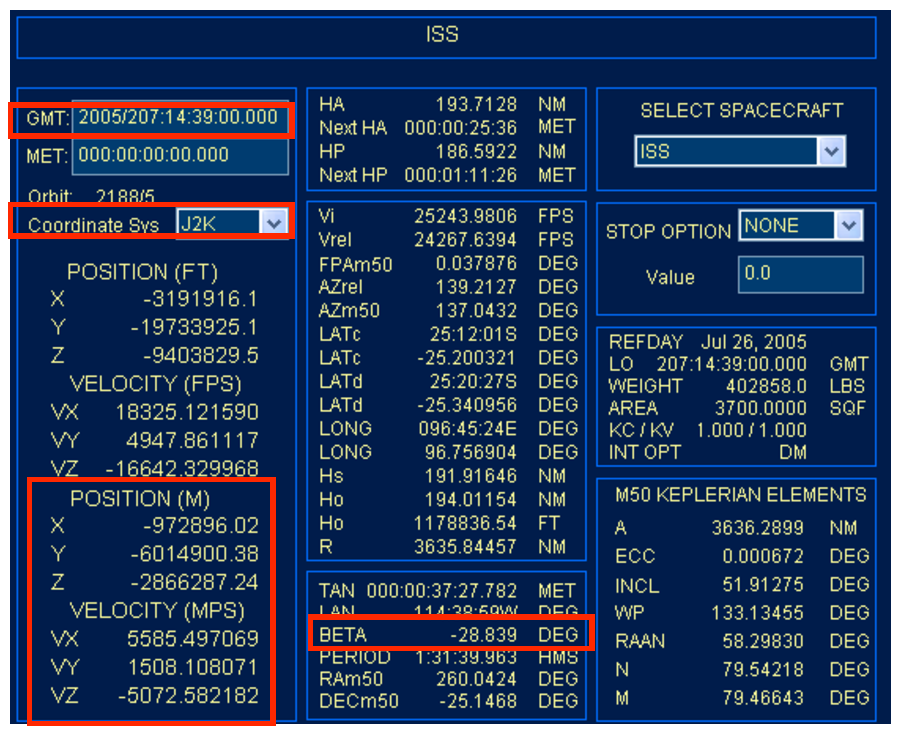
\includegraphics{figures/SOLAR_BETA_fig5}
\caption{Mission Operations ISS State and Solar Beta}
\label{fig:STS_114_ISS}
\end{figure}

\item{RUN\_comp\_STS121a and RUN\_comp\_STS121b] STS-121} \ \newline
These runs compare against the Solar Beta for ISS, generated using the DE405 ephemeris
The Mission Operations Directorate uses the DE405 ephemeris
to compute solar beta angles in flight-certified applications.
Mission STS-121 data, provided by William H. Tracy/NASA/JSC/DM32,
provided solar beta values for a pair of given STS-121 states.

The vehicle state and time as portrayed in
figures~\ref{fig:STS_121a} and~\ref{fig:STS_121b} were used to initialize
the test simulation and to validate the results.
\end{enumerate}

\item{Predictions:}
\begin{enumerate}
\item{RUN\_comp\_ISS} \ \newline
The Solar Beta angles generated by the
simple ephemeris model are accurate to within one degree compared to
angles computed with the aid of the highly accurate DE405 ephemeris model.

Therefore, the solar beta angle computed using the \SolarBetaDesc\ should differ with
the externally-provided value by no more than one degree
for this test case.

\item{RUN\_comp\_STS121a and RUN\_comp\_STS121b}\ \newline
Solar beta angles generated externally using the DE405 ephemeris model
should agree with angles computed by the \SolarBetaDesc\ to a very high degree.
The validation data for these tests provide initial conditions in the M50 reference frame, whereas \JEODid\ uses the J2000 frame.  A conversion of the specification state from M50 to J2000 serves as the initialization data for these tests.  This incorporates a potential source of error.
Other sources of error are in the state vector and the epoch time.
The externally-provided data give solar beta angles with three
decimal places of precision (that is, $1/1000^{th}$ degree).  The initial state and Solar Beta angle for these two tests are shown in Figures~\ref{fig:STS_121a} and~\ref{fig:STS_121b}.

Even accounting for the potential errors introduced by the precision in the specification of the epoch time, and of the M50 state, and further, its conversion to J2000 conversion, the solar beta angle computed using the \SolarBetaDesc\ should differ with the externally-provided value by no more than $0.001^\circ$ for these test cases.
\end{enumerate}

\item{Results:}
\begin{enumerate}
\item{RUN\_comp\_ISS}\\
 The solar beta angle calculated by the simulation at
initialization time was $-28.41^\circ$, which, to within $1^\circ$,
agrees with the externally- supplied value of $-28.839^\circ$.

\item{RUN\_comp\_STS121a and RUN\_comp\_STS121b} \\
The solar beta angles calculated by the simulation at initialization time are
$5.29269^\circ$ (RUN\_comp\_STS121a) and $3.85718^\circ$ (RUN\_comp\_STS121b),
which, to $0.001^\circ$, compare exactly the externally-supplied values
of $5.293^\circ$ and $3.857^\circ$
\end{enumerate}
All test cases pass their respective test criterion.
\end{description}


\begin{figure}
\centering
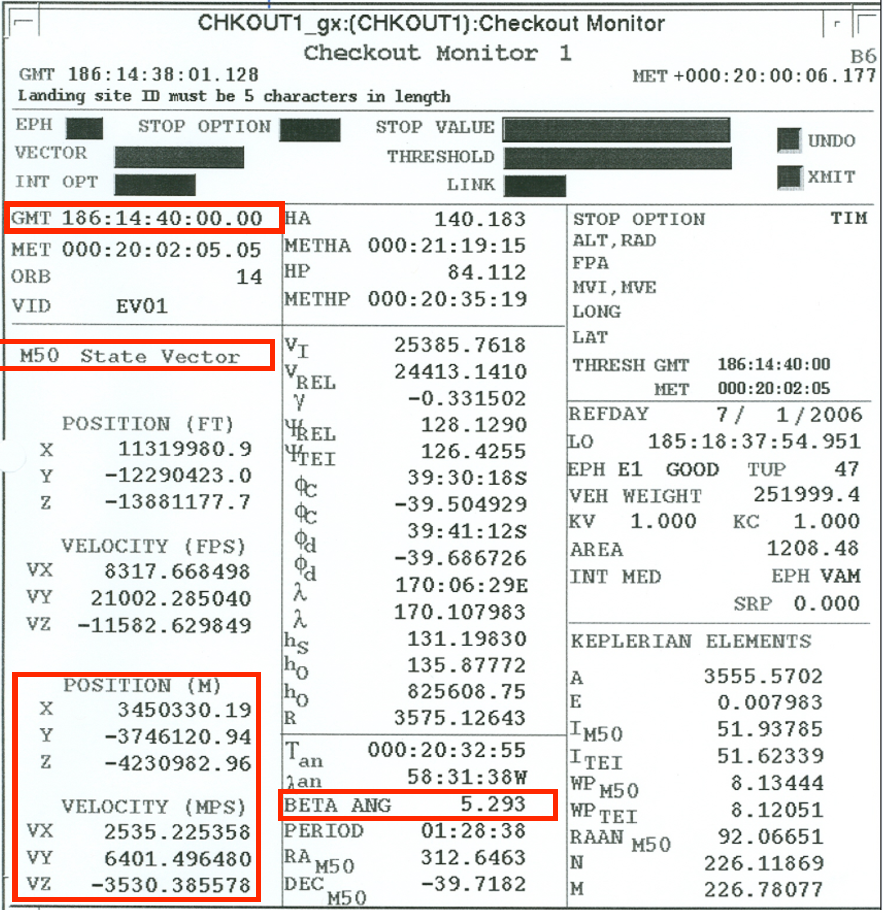
\includegraphics{figures/SOLAR_BETA_fig6}
\caption{Mission Operations STS-121 Checkout Monitor Data}
\label{fig:STS_121a}
\end{figure}


\begin{figure}
\centering
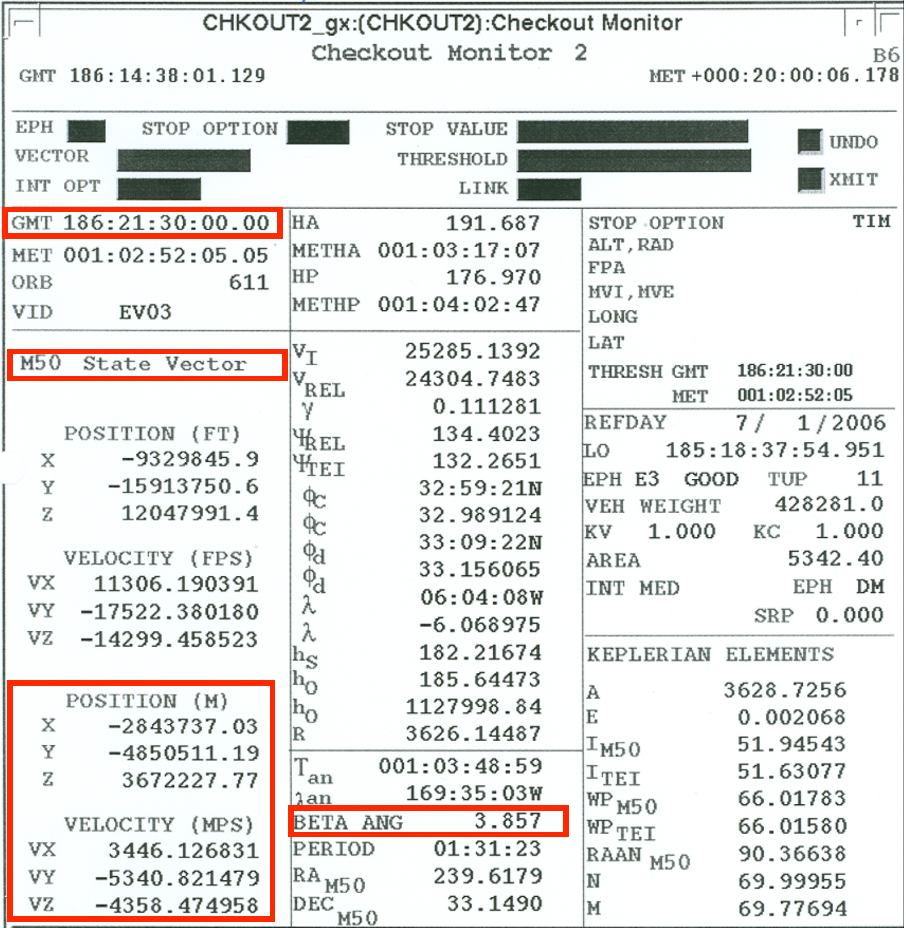
\includegraphics{figures/SOLAR_BETA_fig7}
\caption{Mission Operations STS-121 Checkout Monitor Data}
\label{fig:STS_121b}
\end{figure}

\clearpage



